\documentclass[xcolor=pdflatex,dvipsnames,table]{beamer}

%\documentclass[12pt,handout]{beamer}
%\usepackage{pgfpages}
%\pgfpagesuselayout{4 on 1}[a4paper,border shrink=5mm]


\usepackage{epsfig,graphicx}
\usepackage{palatino}
\usepackage{fancybox}
\usepackage{relsize}
\usepackage[procnames]{listings}

\usepackage{fancyvrb}


\usepackage{times}  % fonts are up to you
\usepackage{graphicx}

\usepackage{algorithm}
\usepackage{algorithmic}
%\usepackage{algpseudocode}
\usepackage{epsfig,subfigure,epstopdf}
\usepackage{amssymb}
%\usepackage{ctex}
\usepackage{amsmath}
\usepackage{listings}

\usepackage{dirtree}

\usepackage{biblatex}
\addbibresource{biblio.bib}


\usepackage{mathtools}

\usepackage{lmodern}


%\documentclass[handout]{beamer}
%\usepackage{pgfpages}
%\pgfpagesuselayout{4 on 1}[a4paper,border shrink=5mm]


% "define" Scala
\usepackage[T1]{fontenc}  
\usepackage[scaled=0.82]{beramono}  
\usepackage{microtype} 

\sbox0{\small\ttfamily A}
\edef\mybasewidth{\the\wd0 }

\lstdefinelanguage{scala}{
  morekeywords={abstract,case,catch,class,def,%
    do,else,extends,false,final,finally,%
    for,if,implicit,import,match,mixin,%
    new,null,object,override,package,%
    private,protected,requires,return,sealed,%
    super,this,throw,trait,true,try,%
    type,val,var,while,with,yield,pr_work,INFINITY},
  sensitive=true,
  morecomment=[l]{//},
  morecomment=[n]{/*}{*/},
  morestring=[b]",
  morestring=[b]',
  morestring=[b]"""
}

\usepackage{color}
\definecolor{dkgreen}{rgb}{0,0.6,0}
\definecolor{gray}{rgb}{0.5,0.5,0.5}
\definecolor{mauve}{rgb}{0.58,0,0.82}

% Default settings for code listings
\lstset{frame=tb,
  language=scala,
  aboveskip=3mm,
  belowskip=3mm,
  showstringspaces=false,
  columns=fixed, % basewidth=\mybasewidth,
  basicstyle={\small\ttfamily},
  numbers=none,
  numberstyle=\footnotesize\color{gray},
  % identifierstyle=\color{red},
  keywordstyle=\color{blue},
  keywordstyle=[2]\color{Purple}, % Perl function arguments purple
  keywordstyle=[3]\color{Blue}\underbar, % Custom functions underlined and blue
  commentstyle=\color{dkgreen},
  stringstyle=\color{mauve},
  frame=single,
  breaklines=true,
  breakatwhitespace=true,
  procnamekeys={def, val, var, class, trait, object, extends},
  procnamestyle=\ttfamily\color{red},
  tabsize=2,
  morekeywords={var,pr_work,INFINITY},
  morekeywords={var,pr_work,INFINITY},
  numbers=left
}

%\lstset{language=C++}
%\lstset{
%  morekeywords={var}
%}


\lstnewenvironment{cpp}[1][]
{\lstset{language=C++,
	morekeywords=[2]{pr_work,INFINITY},
  keywordstyle=[2]\color{dkgreen}, % Perl function arguments purple
#1}}
{}
\lstnewenvironment{scala}[1][]
{\lstset{language=scala,#1}}
{}
\lstnewenvironment{bash}[1][]
{\lstset{language=bash,#1}}
{}
\lstnewenvironment{verilog}[1][]
{\lstset{language=verilog,#1}}
{}


\input{talk.tex}


\input macros.tex

% \def\poster{1}

\title{BLISlab: A Sandbox for Optimizing GEMM}
\author[Jianyu et al]{Jianyu Huang\\Chenhan Yu\\Tyler Smith\\Robert van de Geijn}
\date{\today}
\institute[UT Austin]{SHPC UT Austin\\http://shpc.ices.utexas.edu/}


\AtBeginSection[]  % "Beamer, do the following at the start of every section"
{
\begin{frame}<beamer>
\frametitle{Outline} % make a frame titled "Outline"
\tableofcontents[currentsection]  % show TOC and highlight current section
\end{frame}
}

%% for themes, etc.
%\mode<presentation>
%{ \usetheme{boxes} }


\begin{document}

\begin{frame}
\titlepage
\end{frame}

\section{Introduction}

\subsection{Basic Linear Algebra Subprograms (BLAS)}
\begin{frame}[fragile]
\frametitle{Basic Linear Algebra Subprograms (BLAS)}

\begin{itemize}
\item Standard building blocks for performing vector and matrix operations.
\item Under the hood of high performance scientific applications.
\end{itemize}

 \vskip5mm

{\footnotesize
\centering
{
  \begin{tabular}{c|c|c|c}
  \hline
BLAS category & operations & computation complexity & memory complexity \\
  \hline
BLAS1 & vector-vector & $O(n)$ & $ O(n)$ \\
BLAS2 & matrix-vector & $O(n^2)$ & $O(n^2)$ \\
{\color{red} BLAS3} & matrix-matrix & $O(n^3)$ & $O(n^2)$ \\
  \hline
\end{tabular}
}

}

\end{frame}

\subsection{Matrix-matrix multiplication (\Gemm)}
\begin{frame}[fragile]
\frametitle{Matrix-matrix multiplication (\Gemm)}
\begin{itemize}
\item \Gemm\ is supported by BLAS with the call
\begin{verbatim}

      dgemm( transa, transb, m, n, k,
             alpha, A, lda, B, ldb,
             beta, C, ldc )

\end{verbatim}
\item By appropriately choosing {\tt transa} and {\tt transb},
{\tt dgemm} computes
\[
C := \alpha A B + \beta C; \quad
C := \alpha A^T B + \beta C; \quad
\]
\[
C := \alpha A B^T + \beta C; \quad
C := \alpha A^T B^T + \beta C.
\]
Here $ C $ is $ m \times n $ and $ k $ is the ``third dimension''.

\item We consider the simplified version of \Gemm,
\[
C := A B + C,
\]
where $ C $ is $ m \times n $,
$ A $ is $ m \times k $, and $ B $ is $ k \times n $
\end{itemize}

\end{frame}

\subsection{High-performance implementation}
\begin{frame}[fragile]
\frametitle{High-performance implementation}

  \begin{columns}
	\column{0.5\textwidth}
\centering
{
{\footnotesize
  \begin{tabular}{c|c}
  \hline
Vendors & BLAS library name \\
  \hline
Intel & MKL \\
AMD   & ACML \\
Cray  & LibSci \\
IBM   & ESSL \\
\hline
Nvidia & cublas \\
AMD    & clblas \\
\hline
\end{tabular}
}
}
	\column{0.3\textwidth}
Open Source:\\
ATLAS\\
\textbf{GotoBLAS}: from UT\\
OpenBLAS\\
\textbf{BLIS}:from UT
\end{columns}

\end{frame}


\subsection{Other similar exercises}
\begin{frame}[fragile]
\frametitle{Other similar exercises}
\begin{itemize}

\item \myhref{http://apfel.mathematik.uni-ulm.de/~lehn/sghpc/gemm/index.html}{GEMM: From Pure C to SSE Optimized Micro Kernels} by Michael Lehn
\item \myhref{http://wiki.cs.utexas.edu/rvdg/OptimizingGemm}{Optimizing Gemm} by Robert van de Geijn
\end{itemize}

\end{frame}

\subsection{We need you! HPC's Got Talent!}
\begin{frame}[fragile]
\frametitle{We need you! HPC's Got Talent!}

\begin{itemize}
\item The purpose of this tutorial is to guide you towards high-performance
implementation of \Gemm.

\item Our ulterior motive is that our BLIS framework for implementing BLAS requires a so-called micro-kernel to be highly optimized for various CPUs.

\item In teaching you the basic techniques, we are hoping to identify  ``The One'' who will contribute the best micro-kernel.

\item Our BLIS library supports architectures that include x86 processors by AMD and Intel, IBM's Power processors, ARM processors, and DSP processors.
\end{itemize}

\end{frame}

\section{Step 1: The Basics}
\subsection{Simple matrix-matrix multiplication}
\begin{frame}[fragile]
\frametitle{Simple matrix-matrix multiplication}
$$C:=AB + C$$
where $A$, $B$, and $C$ are $m\times k$, $k\times n$, $m\times n$  matrices, respectively.
Letting
{\footnotesize%
\[
A =
\left( \begin{array}{c c c c}
\alpha_{0,0} & ... & \alpha_{0,k-1} \\
\vdots &  & \vdots \\
\alpha_{m-1,0} & ... & \alpha_{m-1,k-1} \\
\end{array}
\right),
B =
\left( \begin{array}{c c c c}
\beta_{0,0} & ... & \beta_{0,n-1} \\
\vdots &  & \vdots \\
\beta_{k-1,0} & ... & \beta_{k-1,n-1} \\
\end{array}
\right),
\]
\[
C =
\left( \begin{array}{c c c c}
\gamma_{0,0} & ...  & \gamma_{0,n-1} \\
\vdots &  & \vdots \\
\gamma_{m-1,0} & ... & \gamma_{m-1,n-1} \\
\end{array}
\right)
\]%
}

$ C := A B + C $ computes
\[
\gamma_{i,j} := \sum_{p=0}^{k-1} \alpha_{i,p} \beta_{p,j} +
\gamma_{i,j}.
\]
\end{frame}

\begin{frame}[fragile]
\frametitle{Simple matrix-matrix multiplication (Continues)}
If $ A $, $ B $, and $ C $ are stored  in two-dimensional arrays {\tt
  A}, {\tt B}, and {\tt C},
the following pseudocode computes $ C := A B + C $:

\vspace{0.1in}
\begin{center}
\begin{minipage}{4in}
\begin{verbatim}
for i=0:m-1
   for j=0:n-1
      for p=0:k-1
         C( i,j ) := A( i,p ) * B( p,j ) + C( i,j )
      endfor
   endfor
endfor
\end{verbatim}
\end{minipage}
\end{center}
\vspace{0.1in}
Counting a multiply and an add separately,
the computation requires $ 2 m n k $  floating point operations (flops).
\end{frame}

\subsection{Setup}

\begin{frame}[fragile]
\frametitle{Setup}
\begin{itemize}
\item Structure of directory {\tt step1}
\item Configure on {\tt sourceme.sh}
\item Compile, execute and collect result
\item Draw the performance graph
\end{itemize}
\end{frame}

\begin{frame}[fragile]
\frametitle{Leading Dimension}

\begin{verbatim}

   #define C( i, j ) C[ (j)*ldc + (i) ]

\end{verbatim}

\begin{center}
	\includegraphics[width=4in]{figures/LeadingDims.pdf}
\end{center}


\begin{verbatim}

      bl_dgemm( m, n, k, A, lda, B, ldb, C, ldc )

\end{verbatim}

\end{frame}

\begin{frame}[fragile]
\frametitle{Performnce Graph}

\begin{columns}
\column{0.33\textwidth}
\begin{center}
\includegraphics[width=2in]{figures/step1_st_ivy.eps}
\end{center}
\column{0.33\textwidth}
\begin{center}
\includegraphics[width=2in]{figures/step2_st_ivy.eps}
\end{center}
\column{0.33\textwidth}
\begin{center}
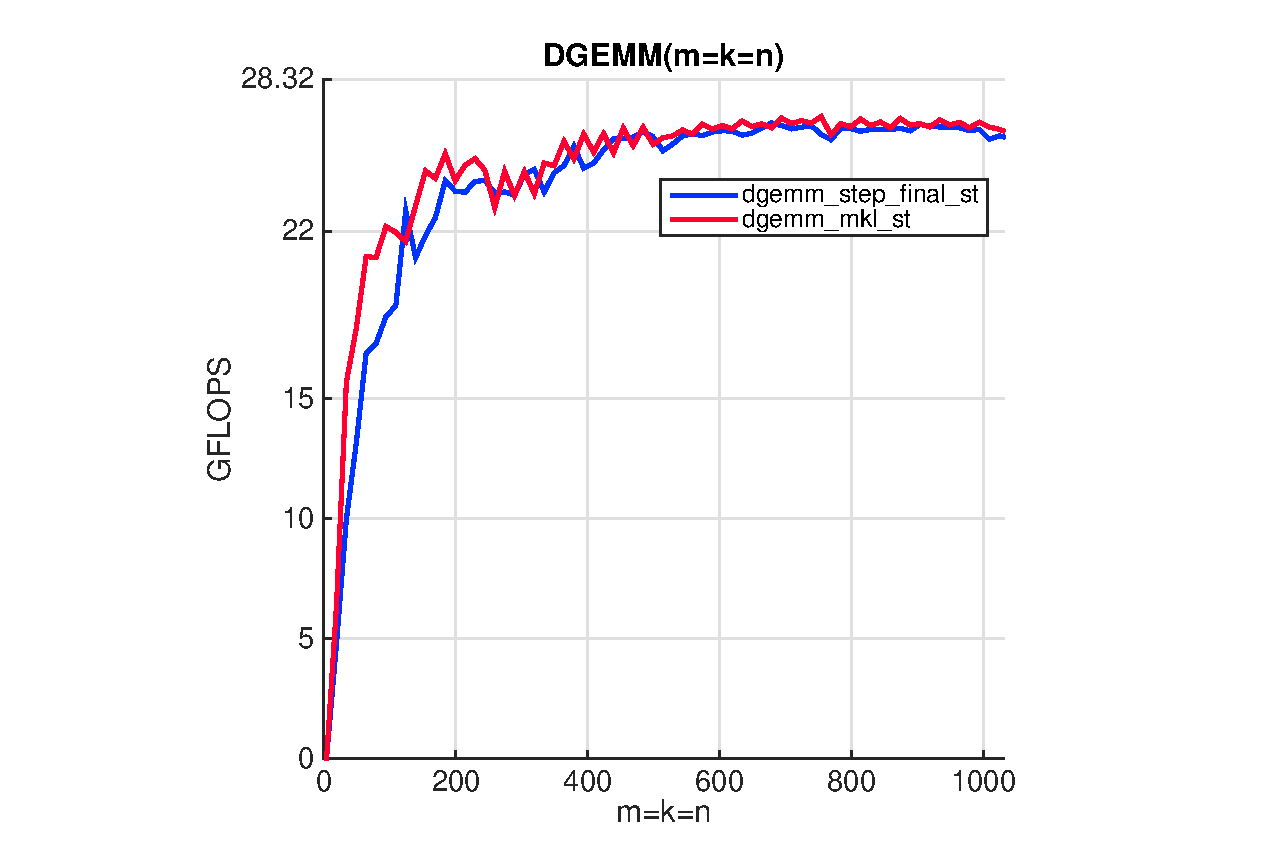
\includegraphics[width=2in]{figures/step3_st_ivy.eps}
\end{center}
\end{columns}

\end{frame}


\subsection{Basic techniques}

\subsubsection{Using pointers}
\begin{frame}[fragile]
\frametitle{Using pointers}

\begin{columns}
\column{0.5\textwidth}
\begin{Verbatim}[frame=single]

for ( i = 0; i < m; i ++ ) {
   for ( j = 0; j < n; j ++ ) {
      C( i, j ) = 0.0;
   }
}

\end{Verbatim}
\column{0.5\textwidth}
\centering{
\begin{Verbatim}[frame=single]

double *cp;
for ( j = 0; j < n; j ++ ) {
   cp = &C[ j * ldc ];
   for ( i = 0; i < m; i ++ ) {
      *cp++ = 0.0;
   }
}

\end{Verbatim}
}
\end{columns}

Notice that we purposely exchanged the order of the loops so that advancing the pointer takes us down the columns of $ C $.

\end{frame}

\subsubsection{Loop unrolling}
\begin{frame}[fragile]
\frametitle{Loop unrolling}

Updating loop index {\tt i} and the pointer {\tt cp} every time through the inner loop creates considerable overhead.  For this reason, a compiler will perform {\em loop unrolling}.  Using an unrolling factor of four, our simple loop for setting {\tt C} to zero becomes
\begin{Verbatim}[frame=single]
double *cp;

for ( j = 0; j < n; j ++ ) {
   cp = &C[ j * ldc ];
   for ( i = 0; i < m; i += 4 ) {
      *(cp+0) = 0.0;
      *(cp+1) = 0.0;
      *(cp+2) = 0.0;
      *(cp+3) = 0.0;
      cp += 4;
      }
   }
}
\end{Verbatim}
\end{frame}

\begin{frame}[fragile]
\frametitle{Loop unrolling}

Importantly:
\begin{itemize}
	\item {\tt i} and {\tt cp} are now only updates once every four iterations.
	\item {\tt *(cp+0)} uses a machine instruction known as {\em indirect addressing} that is much more efficient than if one computed with {\tt *(cp+k)} where $ k $ is a variable.
	\item
	When data it brought in for memory into cache, it is brought in a cache line of 64 bytes at a time.  This means that accessing contiguous data in chunks of 64 bytes reduces the cost of memory movement between the memory layers.
\end{itemize}
Notice that when you unroll, you may have to deal with a ``fringe'' if, in this case, {\tt m} is not a multiple of four.

\end{frame}

\subsubsection{Register variables}
\begin{frame}[fragile]
\frametitle{Register variables}

\begin{Verbatim}[frame=single]
   double *cp;

   for ( j = 0; j < n; j ++ ) {
      cp = &C[ j * ldc ];
      for ( i = 0; i < m; i += 4 ) {
         register double c0=0.0, c1=0.0, c2=0.0, c3=0.0;
         *(cp+0) = c0;
         *(cp+1) = c1;
         *(cp+2) = c2;
         *(cp+3) = c3;
         cp += 4;
      }
   }
\end{Verbatim}

\end{frame}

\subsubsection{Vector intrinsics}
\begin{frame}[fragile]
\frametitle{Vector intrinsics}
\begin{itemize}
\item \myhref{https://software.intel.com/sites/landingpage/IntrinsicsGuide/}{Intel Intrinsics Guide}
\item \myhref{https://software.intel.com/en-us/isa-extensions}{Intel ISA Extensions}
\end{itemize}
\end{frame}

%\section{Vector intrinsics}
\begin{frame}[fragile]
\frametitle{Project}

\begin{Verbatim}[frame=single]

      bl_dgemm( m, n, k, A, lda, B, ldb, C, ldc )

\end{Verbatim}

\end{frame}




\end{document}


